\section{Problem Statement}
% \textit{Outline the problem statement (5), the mathematical model (5), and the computational model parameters (5). In your report, provide the geometry of the simulation domain, governing equations, and mathematical formulation of boundary and initial conditions. In computational model section, present the mesh of the simulation domain (only one mesh out of five), the values of boundary and initial conditions, convergence criteria is set for RMS of momentum at $10^{-5}$, provide the name and order of the scheme used for convective term discretization (should be second order accurate). Use the coupled solver. In a table, list all the models that you selected in “Methods” tab of the software, as well as the details of the solver under “General”.}

\subsection{Objective}
The problem objective is to calculate the drag coefficient $C_d$ of a square object at a Reynolds number of 20 and estimate the length of a vortex that forms behind the object. 

Secondary objectives include learning about mesh refinement and mesh convergence. The problem will be solved numerically in ANSYS Fluent for five systematically refined meshes. The first (coarsest) mesh should contain in the order of 2000-3000 cells or control volumes with a cell size of 5.0 mm. The rest of the meshes are generated by reducing the size of each cell by two in both directions, i.e. increasing the total number of cells by four. The topology of the mesh remains the same as the mesh is refined. During the simulation, it is necessary to monitor the drag force $F_d$ as a function of iteration.

\subsection{Mathematical Model}
\subsubsection{Flow Description}
For the mathematical description of fluids, the Navier-Stokes equations are an appropriate description of the flow. The continuity equation is given by
\begin{align*}
    \frac{\partial}{\partial t} (\rho \vec{v}) + \nabla \cdot (\rho \vec{v} \vec{v}) &= 0
\end{align*}
the momentum equation is 
\begin{align*}
    \frac{\partial}{\partial t} (\rho \vec{v}) + \nabla \cdot (\rho \vec{v} \vec{v}) &= -\nabla p + \frac{1}{3} \mu \nabla (\nabla \cdot \vec{v}) + \mu \nabla^2 \vec{v} + \rho \vec{b}
\end{align*}
There are some simplifications that can be made to the Navier-Stokes equations. Noting that the Reynolds number is low ($\text{Re} \ll 100$), the unsteady and convective terms can be neglected. The flow is also incompressible, so the density is constant. The continuity equation simplifies to
\begin{align*}
    \Aboxed{\nabla \cdot \vec{v} &= 0}
\end{align*}
The momentum equation simplifies to
\begin{align*}
    \Aboxed{\mu \nabla^2 \vec{v} - \nabla p + \rho \vec{g} &= 0}
\end{align*}

\subsubsection{Boundary Conditions}
The boundary conditions for the problem are listed in Table \ref{tab:boundary_conditions}.
\begin{table}[H]
    \centering
    \caption{Boundary Conditions}
    \label{tab:boundary_conditions}
    \begin{tabular}{ll}
        \toprule
        Boundary & Condition \\
        \midrule
        Inlet & $\displaystyle u|_{\text{inlet}} = U_\infty = 0.04$ m/s \\[2ex]
        Outlet & $\displaystyle \frac{\partial u}{\partial x}\bigg|_{\text{outlet}} = 0$ \\[2ex]
        Top and Bottom Walls & $\displaystyle \mu \frac{\partial u}{\partial y}\bigg|_{\pm 10D} = 0$ \\[2ex]
        Square Wall & $\displaystyle \vec{v}|_{\text{square}} = 0$ \\
        \bottomrule
    \end{tabular}
\end{table}

\subsection{Computational Model Parameters}
\subsection{Geometry and Mesh}
\begin{figure}[H]
    \centering
    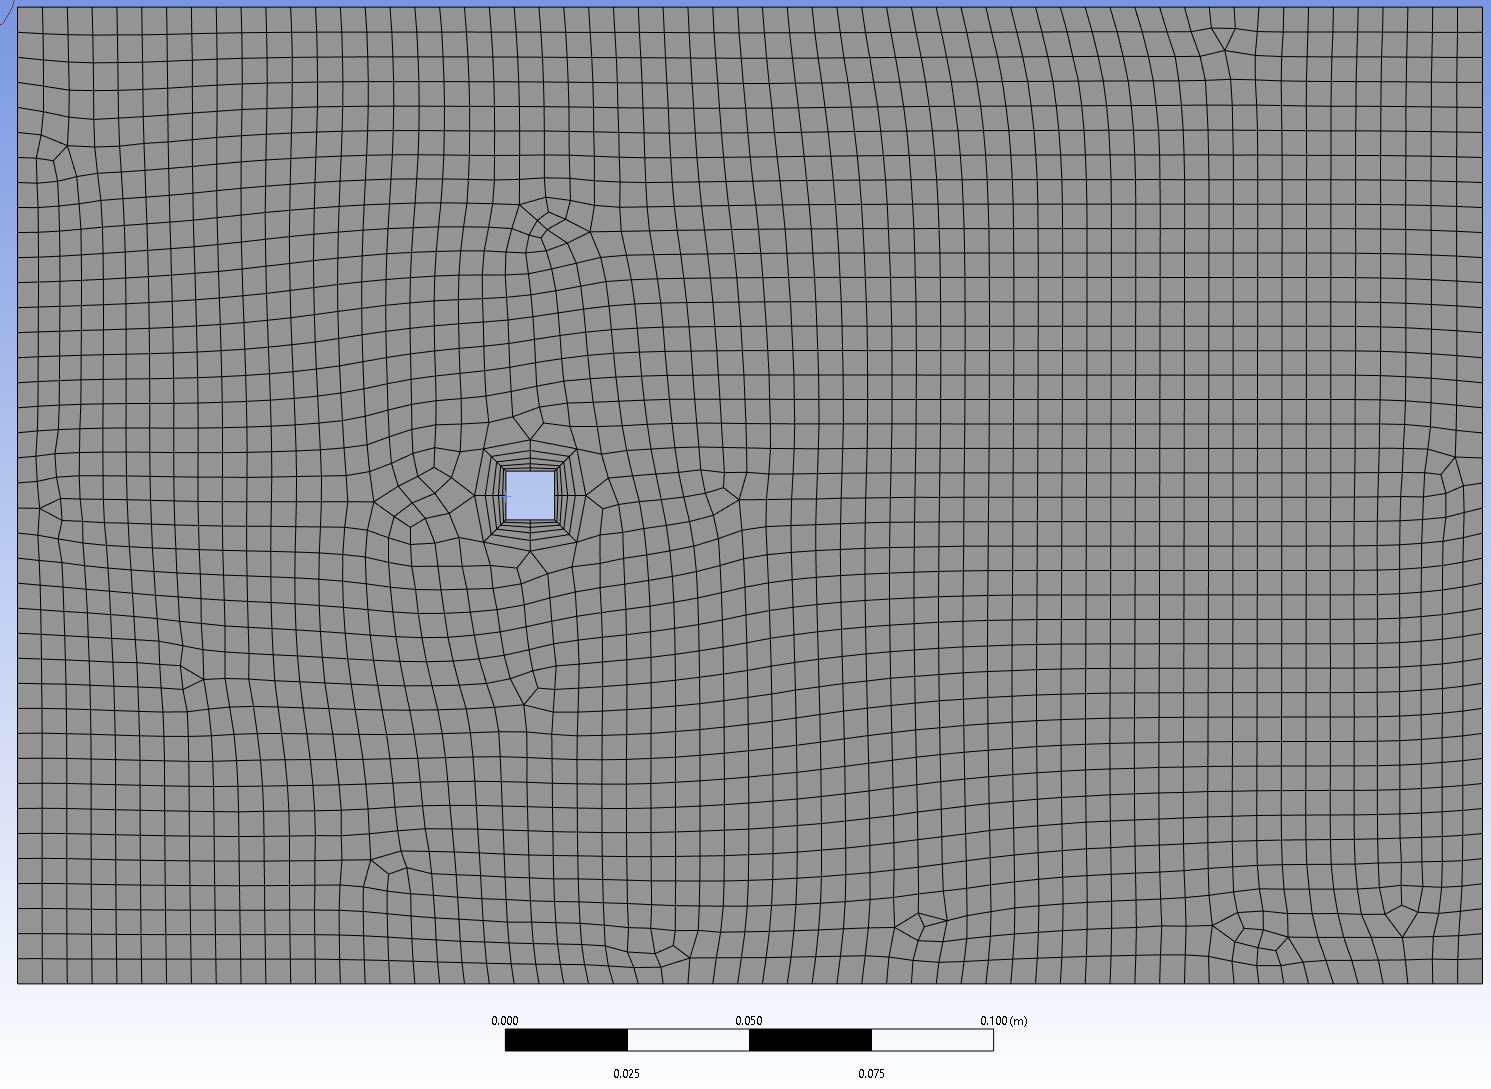
\includegraphics[width=0.5\textwidth]{Questions/Figures/grid 1 mesh.png}
    \caption{Geometry and Mesh for Mesh 1}
    \label{fig:mesh1}
\end{figure}
The geometry of the simulation domain is a square object with side length $D = 0.01$ m. The domain is 0.2 m long and 0.1 m tall. 

Face sizing was used with 5 inflation layers around the square with a growth rate of 1.2 and a default transition ratio of 0.272. The number of elements in each mesh is shown in Table \ref{tab:mesh_sizes}. The mesh for the first mesh is shown in Figure \ref{fig:mesh1}. 
\begin{table}[H]
    \centering
    \caption{Mesh Sizes}
    \label{tab:mesh_sizes}
    \begin{tabular}{ccc}
        \toprule
        Mesh & Element Size & Number of Elements \\
        & (mm) & \\
        \midrule
        1 & 5.0 & 2390 \\
        2 & 2.5 & 9390 \\
        3 & 1.25 & 37870 \\
        4 & 0.625 & 152044 \\
        5 & 0.3125 & 613378 \\
        \bottomrule
    \end{tabular}
\end{table}

\subsubsection{Boundary Conditions}
First $U_\infty$ needs to be determined. The Reynolds number is given from the problem statement as $Re = 20$. Then,
\begin{align*}
    \text{Re} &= \frac{U_\infty \rho D}{\mu} \\ 
    \implies U_\infty &= \frac{\text{Re} \mu}{\rho D}
\end{align*}
The properties of air are given as $\rho = 1.0$ kg/m$^3$ and $\mu = 2.0 \times 10^{-5}$ kg/m$\cdot$s. The side length of the square object is $D = 0.01$ m. Thus,
\begin{align*}
    U_\infty &= \frac{20 \times 2.0 \times 10^{-5}}{1.0 \times 0.01} = 0.04 \text{ m/s}
\end{align*}
The inlet velocity was specified as $U_\infty = 0.04$ m/s. The outlet boundary condition was specified as zero pressure gradient. The top and bottom walls were specified as no-shear walls. The square wall was specified as a no-slip wall.

\subsubsection{Solver Details}
The solver details are shown in Table \ref{tab:solver_details}.
\begin{table}[H]
    \centering
    \caption{General Solver Details}
    \label{tab:solver_details}
    \begin{tabular}{cc}
        \toprule
        Type & Pressure Based \\
        Velocity Formation & Absolute \\
        Time & Steady \\
        2D Space & Planar \\
        \bottomrule
    \end{tabular}
\end{table}
The convergence criteria for continuity, x-velocity, and y-velocity were set to $10^{-5}$. The spatial discretization scheme is shown in Table \ref{tab:discretization_scheme}. A coupled solver was used. The maximum number of iterations was set to 1000.
\begin{table}[H]
    \centering
    \caption{Discretization Scheme}
    \label{tab:discretization_scheme}
    \begin{tabular}{cc}
        \toprule
        Variable & Scheme \\
        \midrule
        Gradient & Least Squares Cell Based \\
        Pressure & Second Order \\
        Momentum & Second Order Upwind \\
        \bottomrule
    \end{tabular}
\end{table}
% \end{table}
% The mesh element size will be 5.0 mm for the first mesh. The mesh will be refined by reducing the mesh element size by 2, resulting in a total of 4 times the number of cells. The mesh will be refined 5 times. The convergence criteria is set for the RMS of momentum at $10^{-5}$. The scheme used for convective term discretization is second order accurate. The coupled solver will be used.

% 5 inflation layers, growth rate of 1.2, default transition ratio 0.272

% use viscous laminar model 

% describe the BC i guess idk what they want


%     method: coupled
%     Gradient: least squares cell based
%     Pressure: Second order
%     Momentum: Second order upwind

%     start point (0.001, 0.005)
%     end point (0.20005, 0.005)
%     max iterations 1000

%     mesh 1: 2390 elements
%     mesh 2: element size 0.0025, 9390 elements
%     mesh 3: element size 0.00125, 37870 elements
%     mesh 4: element size 0.000625, 152044 elements
%     mesh 5: element size 0.0003125, 613378 elements